\documentclass[9pt]{IEEEtran}

\usepackage[english]{babel}
\usepackage{graphicx}
\usepackage{float}
\usepackage{amsmath}
\usepackage{hyperref}
\usepackage{xcolor}
\usepackage[utf8x]{inputenc}
\usepackage[T1]{fontenc}
\usepackage{lmodern}

\title{\vspace{0ex}Parallel Histogram Equalization Using CUDA}
\author{Erik Pahor, Jaka Škerjanc\vspace{-4.0ex}}

\begin{document}

\maketitle

\section{Introduction}
This project implements parallel histogram equalization for color images using CUDA. Histogram equalization is a contrast enhancement technique that redistributes image luminance to span the entire intensity range. For color images, we operate on the Y (luminance) channel after converting RGB to YUV, to avoid altering color tones.

The process includes: converting RGB to YUV, computing the luminance histogram, calculating the cumulative distribution function (CDF), equalizing pixel intensities, and converting the image back to RGB.

We implemented a sequential CPU version, a parallel CUDA version with atomic operations and an optimized CUDA version using shared memory and partial histograms to reduce contention.

All stages were offloaded to the GPU with minimal host-device memory transfers to maximize performance.

\section{Implementation Details}

\subsection{RGB to YUV Conversion}
This transformation is applied in parallel: one thread per pixel. Each thread computes Y, U, and V using matrix multiplication. Only the Y component is processed for equalization.

\subsection{Histogram Computation}
The baseline CUDA implementation uses a global histogram updated with \texttt{atomicAdd}. However, atomic contention becomes a bottleneck for high-resolution images.

To optimize this, we allocate shared memory per thread block to store partial histograms. Each thread updates the local shared histogram, reducing global memory atomics. After synchronization, block histograms are atomically merged into the global histogram.

\subsection{CDF and Lookup Table}
We first implemented a simple CDF computation using a single GPU thread. For the bonus version, we applied Blelloch’s work-efficient scan algorithm to parallelize this stage, leveraging shared memory and thread synchronization.

The final lookup table (LUT) maps old luminance values to new ones using:
\[
l' = \frac{CDF(l) - CDF_{min}}{(N \times M - CDF_{min})} \times (L - 1)
\]
This LUT is stored in global memory and reused during intensity remapping.

\subsection{Applying the LUT}
Each pixel’s Y value is replaced using the LUT. Threads operate independently, making this step highly parallelizable. The final YUV image is converted back to RGB in parallel.

\section{Experimental Results}
We tested the three implementations on images of various resolutions. Each result is averaged over 7 runs. Table~\ref{tab:avg_times} shows the average execution times.

\begin{table}[H]
\centering
\begin{tabular}{|c|c|c|c|}
\hline
Image Size & Sequential & Parallel & Optimized \\ \hline
720x480   & 14.60 ms  & 0.74 ms  & 0.47 ms  \\ \hline
1024x768  & 29.25 ms  & 1.00 ms  & 0.75 ms  \\ \hline
1920x1200 & 80.46 ms  & 3.14 ms  & 1.61 ms  \\ \hline
3840x2160 & 274.34 ms & 7.75 ms  & 4.04 ms  \\ \hline
7680x4320 & 989.65 ms & 31.53 ms & 15.23 ms \\ \hline
\end{tabular}
\caption{Average execution times for each implementation.}
\label{tab:avg_times}
\end{table}

The resulting speed-ups are presented in Table~\ref{tab:speedups}.

\begin{table}[H]
\centering
\begin{tabular}{|c|c|c|}
\hline
Image Size & Parallel Speed-Up & Optimized Speed-Up \\ \hline
720x480   & 19.7\(\times\)   & 31.0\(\times\) \\ \hline
1024x768  & 29.3\(\times\)   & 39.3\(\times\) \\ \hline
1920x1200 & 25.6\(\times\)   & 49.9\(\times\) \\ \hline
3840x2160 & 35.4\(\times\)   & 67.9\(\times\) \\ \hline
7680x4320 & 31.4\(\times\)   & 65.0\(\times\) \\ \hline
\end{tabular}
\caption{Speed-up factors relative to the sequential version.}
\label{tab:speedups}
\end{table}

\begin{figure}[H]
    \centering
    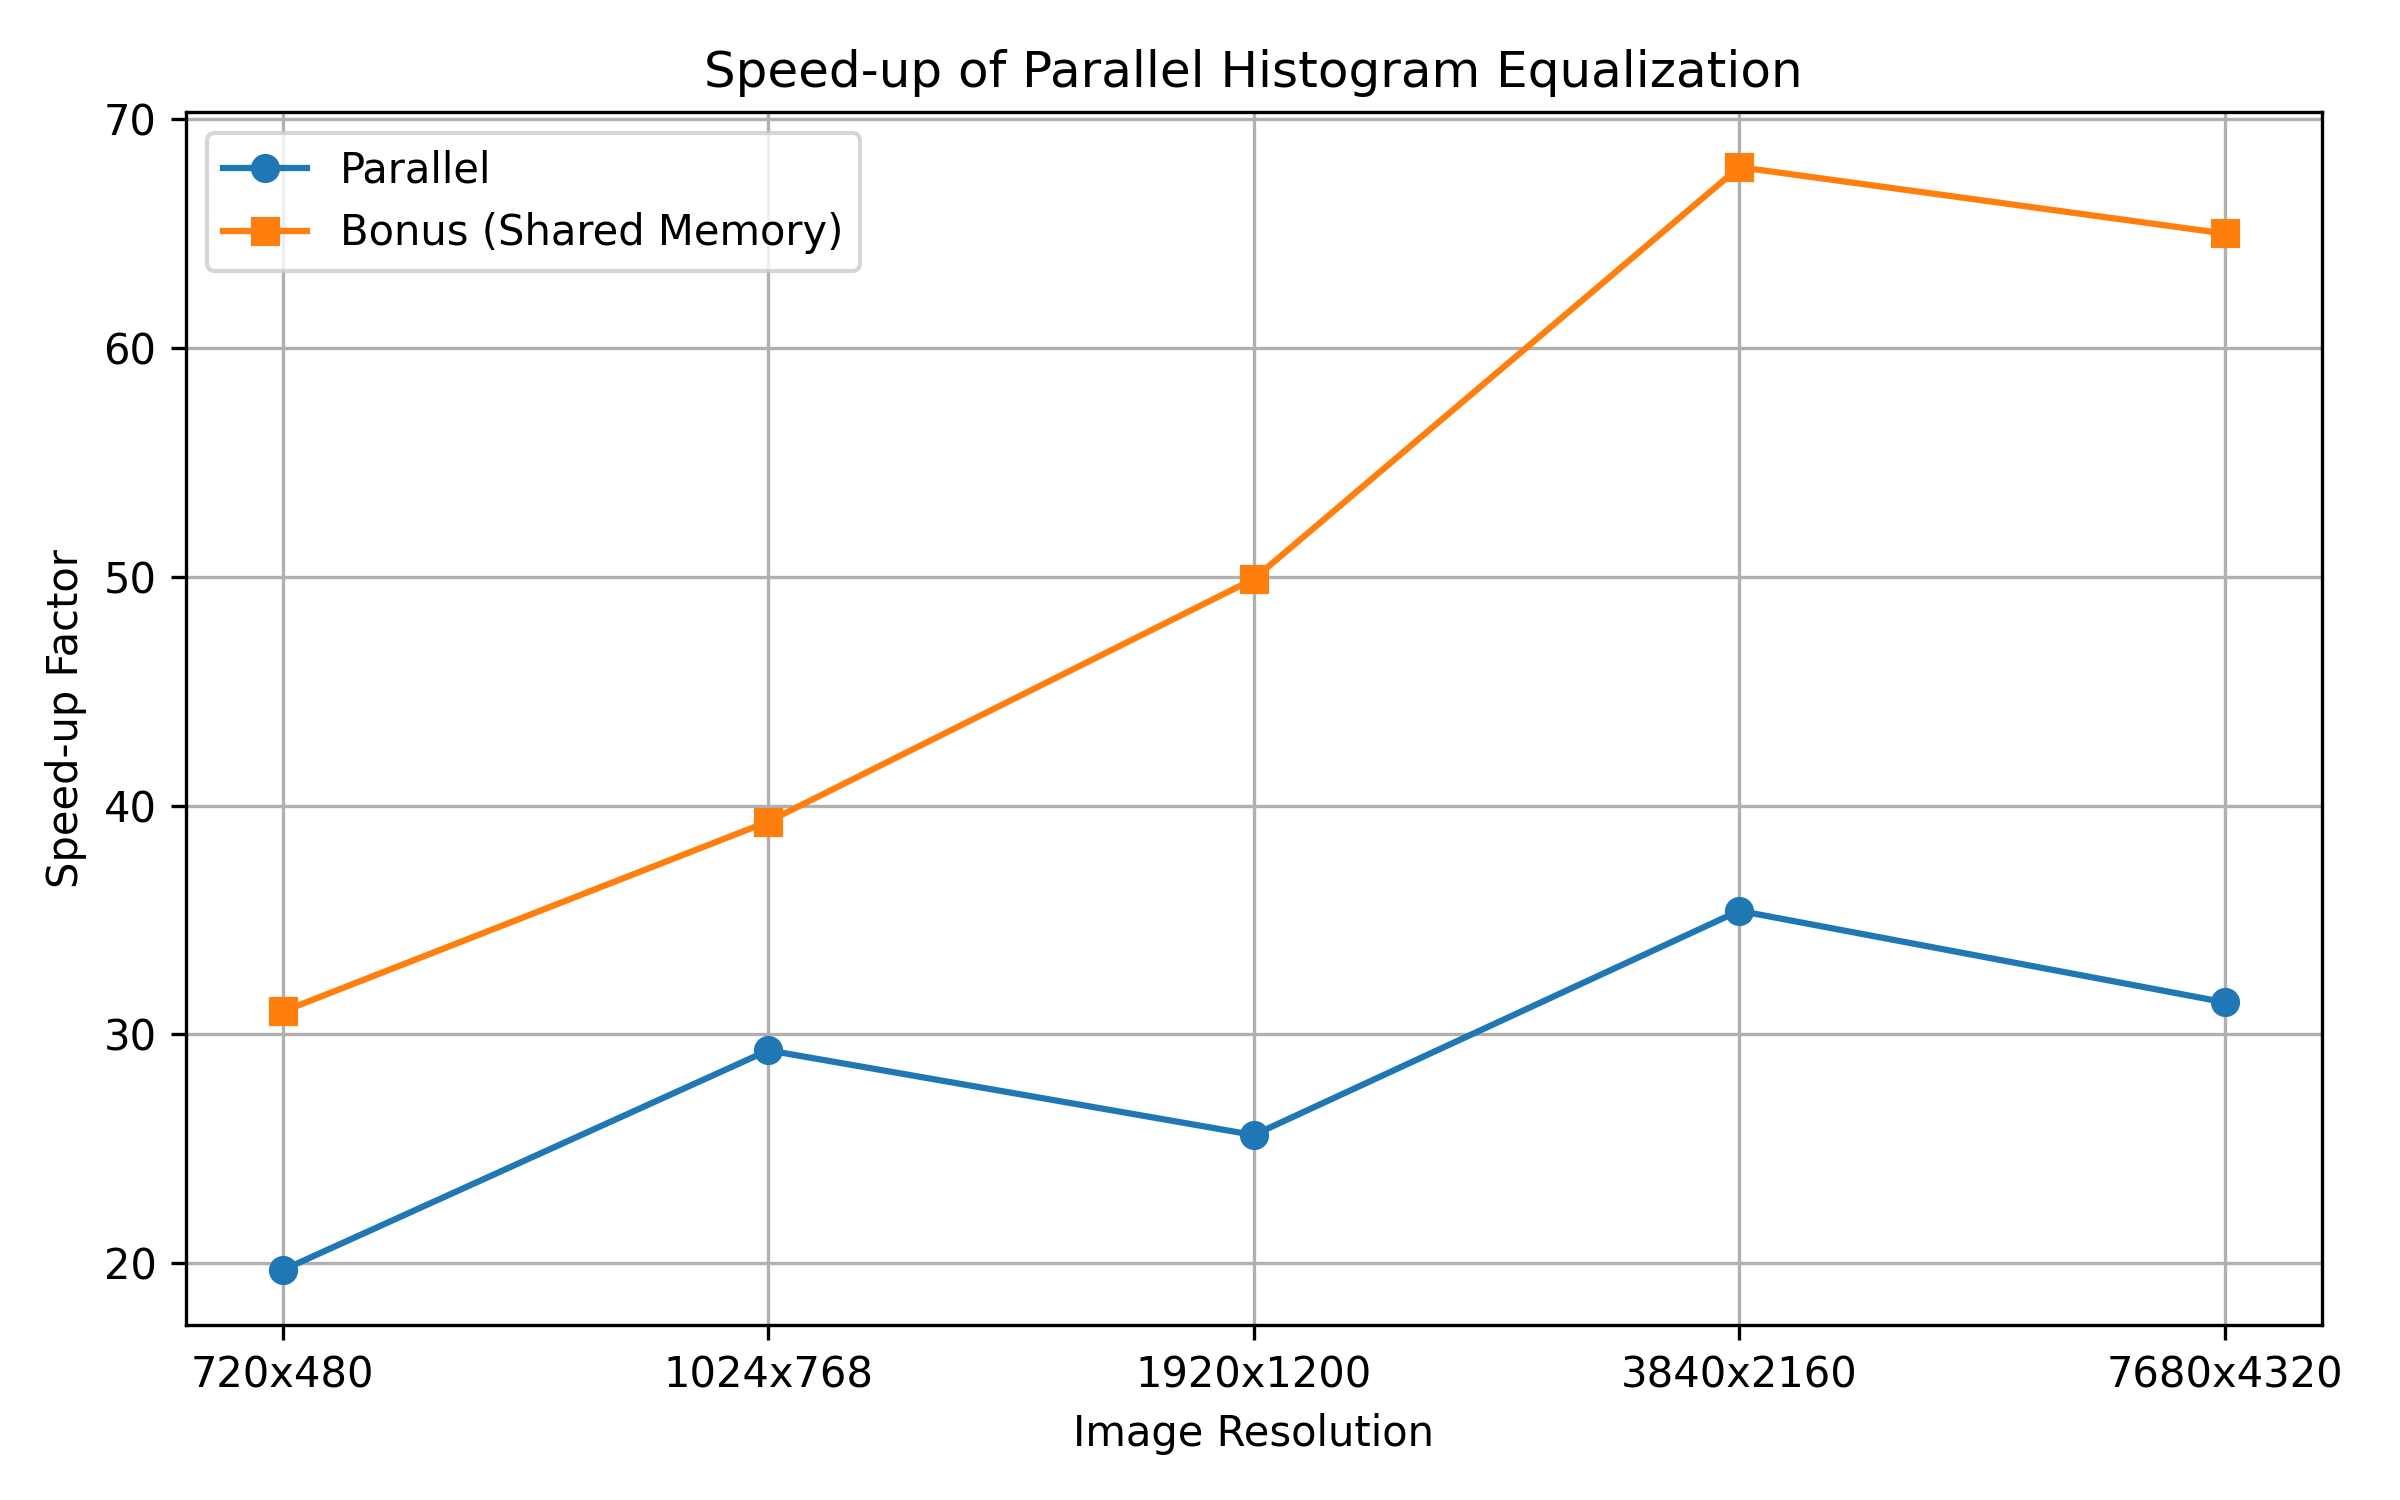
\includegraphics[width=0.9\columnwidth]{speedup.png}
    \caption{Speed-up of parallel and optimized CUDA implementations.}
    \label{fig:speedup}
\end{figure}

\section{Discussion}
Significant speed-ups were observed, especially at higher resolutions where GPU parallelism is better utilized. The baseline CUDA version suffers from atomic contention in histogram computation. Introducing shared memory in the optimized version drastically reduced contention and improved memory coalescing.

The use of partial histograms per thread block greatly reduced global memory atomic operations. For the CDF stage, the parallel prefix sum (scan) reduced runtime compared to the naive implementation, though benefits here were modest due to the small size (256 bins).

Overall, optimizations targeting memory hierarchy and minimizing contention had the greatest impact on performance.

\section{Conclusion}
We demonstrated a full GPU-accelerated histogram equalization algorithm for color images using CUDA. Optimizations such as shared memory usage, partial histograms, and work-efficient scan significantly improved performance. For large images, our optimized version achieved speed-ups exceeding 65\(\times\) over the sequential version.

Future improvements could include overlapping computation and data transfer with CUDA streams or exploring warp-level primitives for even finer control.

\bibliographystyle{IEEEtran}
\bibliography{bibliography}

\end{document}
